\tikzset{every picture/.style={line width=0.75pt}} %set default line width to 0.75pt        

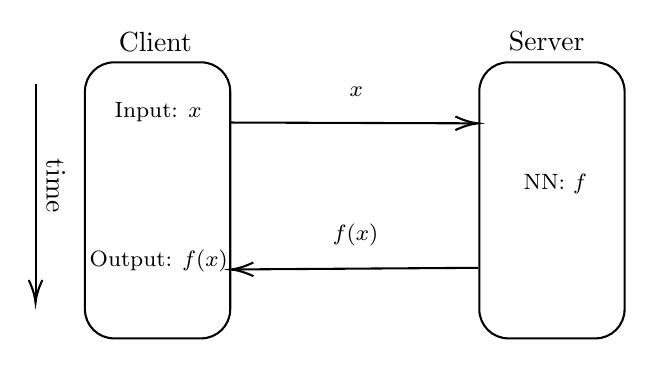
\begin{tikzpicture}[x=0.75pt,y=0.75pt,yscale=-1,xscale=1]
    %uncomment if require: \path (0,300); %set diagram left start at 0, and has height of 300
    
    %Rounded Rect [id:dp8363217487457562] 
    \draw   (29.2,33.2) .. controls (29.2,25.47) and (35.47,19.2) .. (43.2,19.2) -- (85.2,19.2) .. controls (92.93,19.2) and (99.2,25.47) .. (99.2,33.2) -- (99.2,138.2) .. controls (99.2,145.93) and (92.93,152.2) .. (85.2,152.2) -- (43.2,152.2) .. controls (35.47,152.2) and (29.2,145.93) .. (29.2,138.2) -- cycle ;
    %Straight Lines [id:da5921212328183769] 
    \draw    (99,48.2) -- (216.6,48.59) ;
    \draw [shift={(218.6,48.6)}, rotate = 180.19] [color={rgb, 255:red, 0; green, 0; blue, 0 }  ][line width=0.75]    (10.93,-3.29) .. controls (6.95,-1.4) and (3.31,-0.3) .. (0,0) .. controls (3.31,0.3) and (6.95,1.4) .. (10.93,3.29)   ;
    %Rounded Rect [id:dp06719723111527287] 
    \draw   (219.2,33.2) .. controls (219.2,25.47) and (225.47,19.2) .. (233.2,19.2) -- (275.2,19.2) .. controls (282.93,19.2) and (289.2,25.47) .. (289.2,33.2) -- (289.2,138.2) .. controls (289.2,145.93) and (282.93,152.2) .. (275.2,152.2) -- (233.2,152.2) .. controls (225.47,152.2) and (219.2,145.93) .. (219.2,138.2) -- cycle ;
    %Straight Lines [id:da8018903239316999] 
    \draw    (218.6,118.2) -- (101.4,118.99) ;
    \draw [shift={(99.4,119)}, rotate = 359.62] [color={rgb, 255:red, 0; green, 0; blue, 0 }  ][line width=0.75]    (10.93,-3.29) .. controls (6.95,-1.4) and (3.31,-0.3) .. (0,0) .. controls (3.31,0.3) and (6.95,1.4) .. (10.93,3.29)   ;
    %Straight Lines [id:da34452920509016227] 
    \draw    (5.4,29.8) -- (5.4,133) ;
    \draw [shift={(5.4,135)}, rotate = 270] [color={rgb, 255:red, 0; green, 0; blue, 0 }  ][line width=0.75]    (10.93,-3.29) .. controls (6.95,-1.4) and (3.31,-0.3) .. (0,0) .. controls (3.31,0.3) and (6.95,1.4) .. (10.93,3.29)   ;
    
    % Text Node
    \draw (44,3.2) node [anchor=north west][inner sep=0.75pt]   [align=left] {Client};
    % Text Node
    \draw (232,3) node [anchor=north west][inner sep=0.75pt]   [align=left] {Server};
    % Text Node
    \draw (155.2,29.6) node [anchor=north west][inner sep=0.75pt]   [align=left] {{\footnotesize $\displaystyle x$}};
    % Text Node
    \draw (42,36.93) node [anchor=north west][inner sep=0.75pt]   [align=left] {{\footnotesize Input: $\displaystyle x$}};
    % Text Node
    \draw (239,71.33) node [anchor=north west][inner sep=0.75pt]   [align=left] {{\footnotesize NN: $\displaystyle f$}};
    % Text Node
    \draw (147.2,95.6) node [anchor=north west][inner sep=0.75pt]   [align=left] {{\footnotesize $\displaystyle f( x)$}};
    % Text Node
    \draw (30,108) node [anchor=north west][inner sep=0.75pt]   [align=left] {{\footnotesize Output: $\displaystyle f( x)$}};
    % Text Node
    \draw (21.1,64.1) node [anchor=north west][inner sep=0.75pt]  [rotate=-90] [align=left] {time};


\end{tikzpicture}
